%%%%%%%%%%%%%%%%%%%%%%%%%%%%%%%%%%%%%%%%%%%%%%%%%%%%%%%%%%%%%%%%%%%%%%%%%%%%%%%%
%2345678901234567890123456789012345678901234567890123456789012345678901234567890
%        1         2         3         4         5         6         7         8

\documentclass[letterpaper, 10 pt, conference]{ieeeconf}  % Comment this line out if you need a4paper

%\documentclass[a4paper, 10pt, conference]{ieeeconf}      % Use this line for a4 paper

\IEEEoverridecommandlockouts                              % This command is only needed if 
                                                          % you want to use the \thanks command

\overrideIEEEmargins                                      % Needed to meet printer requirements.

%In case you encounter the following error:
%Error 1010 The PDF file may be corrupt (unable to open PDF file) OR
%Error 1000 An error occurred while parsing a contents stream. Unable to analyze the PDF file.
%This is a known problem with pdfLaTeX conversion filter. The file cannot be opened with acrobat reader
%Please use one of the alternatives below to circumvent this error by uncommenting one or the other
%\pdfobjcompresslevel=0
%\pdfminorversion=4

% See the \addtolength command later in the file to balance the column lengths
% on the last page of the document

% The following packages can be found on http:\\www.ctan.org
\usepackage{graphics} % for pdf, bitmapped graphics files
\usepackage{epsfig} % for postscript graphics files
%\usepackage{mathptmx} % assumes new font selection scheme installed
%\usepackage{times} % assumes new font selection scheme installed
\usepackage{amsmath} % assumes amsmath package installed
\usepackage{amssymb}  % assumes amsmath package installed
\usepackage{textcomp}
\usepackage{subcaption}
\title{\LARGE \bf
Comparison of Model-Based and Model-Free Reinforcement Learning and Optimal Control
}


\author{Julia Str\"obel, Sebastian H\"ugler, and Jan Br\"udigam}


\begin{document}



\maketitle
\thispagestyle{empty}
\pagestyle{empty}


%%%%%%%%%%%%%%%%%%%%%%%%%%%%%%%%%%%%%%%%%%%%%%%%%%%%%%%%%%%%%%%%%%%%%%%%%%%%%%%%
\begin{abstract}

The control of dynamical systems can be achieved by a variety of approaches with different advantages and drawbacks. In this paper, implementations of model-based reinforcement learning (RL), model-free RL, and optimal control for linear and non-linear dynamical systems are compared and discussed. The results show +one sentence about what results show+

\end{abstract}


%%%%%%%%%%%%%%%%%%%%%%%%%%%%%%%%%%%%%%%%%%%%%%%%%%%%%%%%%%%%%%%%%%%%%%%%%%%%%%%%
\section{INTRODUCTION}

The increase of computational power in recent years has allowed for the successful implementation of learning algorithms to control a wide range of dynamical systems. Nonetheless, classical approaches to control problems also provide 
useful solutions for this class of systems. Therefore, the aim of this paper is to present and discuss algorithms and results, as well as advantages and drawbacks of different control approaches, namely model-based reinforcement learning (RL), model-free RL, and optimal control. These methods are applied to a spring-mass system, a pendulum, and a cart-pole system.

The algorithms and results for the three approaches are presented in Sec. II, Sec. III, and Sec. IV, while a discussion of the findings is provided in Sec. V and a summarizing conclusion is drawn in Sec. VI.

\section{MODELS}
The following three models are controlled by the three different control algorithms:
\subsection{Spring Damper Mass}
The spring-mass system can be described by a system of differential equations
\begin{equation}\label{eqn:JanSMsys}
	\ddot{x}=
	\underbrace{
		\left( {\begin{array}{cc}
			0 &1\\
			-\frac{k}{m} &0\end{array} } \right)}_{A}x + 
	\underbrace{
		\left( {\begin{array}{cc}
		0\\
		\frac{1}{m}\end{array} } \right)}_{B}u,
\end{equation}
with the parameters $k=1$\,N/m (spring) and $m=1$\,kg (mass),
while the output of the system is given as
\begin{equation}\label{eqn:JanSMoutput}
	y=
	\underbrace{
		(1\quad 0)}_{C}x.
\end{equation}
\subsection{Pendulum}
The dynamics of the pendulum are described in (\ref{eqn:JanPsys}).
\begin{equation}\label{eqn:JanPsys}
\dot{x}=
	\left( {\begin{array}{cc}
		x_2\\
		\tfrac{u \: - \: \,b\,x_2 \: - \: m\,g\,s\sin(x_1)}{m\,s^2}\end{array} } \right),
\end{equation}
with the input $u$, the parameters $b=0.2$\,sNm/rad (friction), $m=1$\,kg (mass), $g=9.82$\,m/s$^2$ (gravity), and $s=1$\,m (length of the pendulum).
\subsection{Cart Pole}
The cart-pole dynamics are as follows:
\begin{equation}\label{eqn:JanCPsys}
\dot{x}=
\left( {\begin{array}{cc}
	x_2\\
	\frac{2\,m\,l\,x_4^2\,\text{s}_3 \: + \: 3\,m\,g\,\text{s}_3\,\text{c}_3 \: + \: 4(u \: - \: c\,x_2)}{4(M \: + \: m) \: - \: 3\,m\,\text{c}_3^2}\\
	x_4\\
	\frac{-3\,m\,l\,x_4^2\,\text{s}_3\,\text{c}_3 \: - \: 6(M \: + \: m)\,g\,\text{s}_3 \: - \: 6(u \: - \: c\,x_2)\,\text{c}_3}{l(4(M \: + \: m) \: - \: 3\,m\,\text{c}_3^2)}\end{array} } \right),
\end{equation}
with the parameters $m=0.2$\,kg (mass of pendulum),  $M=1$\,kg (mass of cart), $l=0.5$\,m (length of the pole), $g=9.82$\,m/s$^2$ (gravity), $c=0.2$\,sN/m (friction), and where s$_3$ and c$_3$ stand for sin$(x_3)$ and cos$(x_3)$, respectively.

\subsection{Simulations}
For the comparison of the following algorithms the simulation horizon for all models is 2.5 seconds and the maximum executable force for the spring damper mass and cart pole is 10 N and the maximum torque for the pendulum is 10 Nm. The initial state of spring damper mass (pendulum) is 0 m (0\textdegree) and 0 $\frac{m}{s}$ (0$\frac{rad}{s}$). The cart pole starts at the initial angles 10\textdegree , 90\textdegree and 180\textdegree and zero position of the cart. 
%(For comparison the control energy is obtained by cumulative squared control input and the cost of the trajectory is the cumulative square of state variables.)

\section{MODEL-BASED RL}
In model based reinforcement learning a model of the system to be controlled is learned using measurement data. Secondly a policy is optimized using the learned model in order to control the real world system afterwards.

%In a model based reinforcement approach a model is trained at first using data sampled of a real world system. The data is generated by applying a policy on the system. %At first a random and afterwards optimized policies are used. 
%Having trained the artificial model, closed loop simulations using this model are done in order to optimize the policy moving the system to its target state.%, which is necessary to move the model to a predefined target state.
%%+Maybe a few sentences about the general idea/concept of model-based RL+
\subsection{Algorithm}
In this work the PILCO %(Probabilistic Inference for Learning COntrol)
approach for model based reinforcement learning presented in \cite{PILCO_paper} is investigated.% and a rough overview over the algorithm is given.
\newline In PILCO a probabilistic dynamic model for long term policy planning is trained. The unknown system dynamics are assumed with 
\begin{equation}\label{PILCO_sysEq}
x_t = f\left(x_{t-1},u_{t-1}\right)
\end{equation}
where $x\in \mathbb{R}^D$ are the real valued system states, $u \in \mathbb{R}^U$ are the control inputs and $f$ is the unkown transition dynamics. The aim of PILCO is to find a policy $\pi$ for the unkown system, i.e. the optimal parameters $\theta$ of a controller, to minimize a cumulative cost $J^\pi\left(\theta\right)$. 

\begin{figure*}[!thp] 
	\centering
	\begin{subfigure}{0.325\textwidth}
	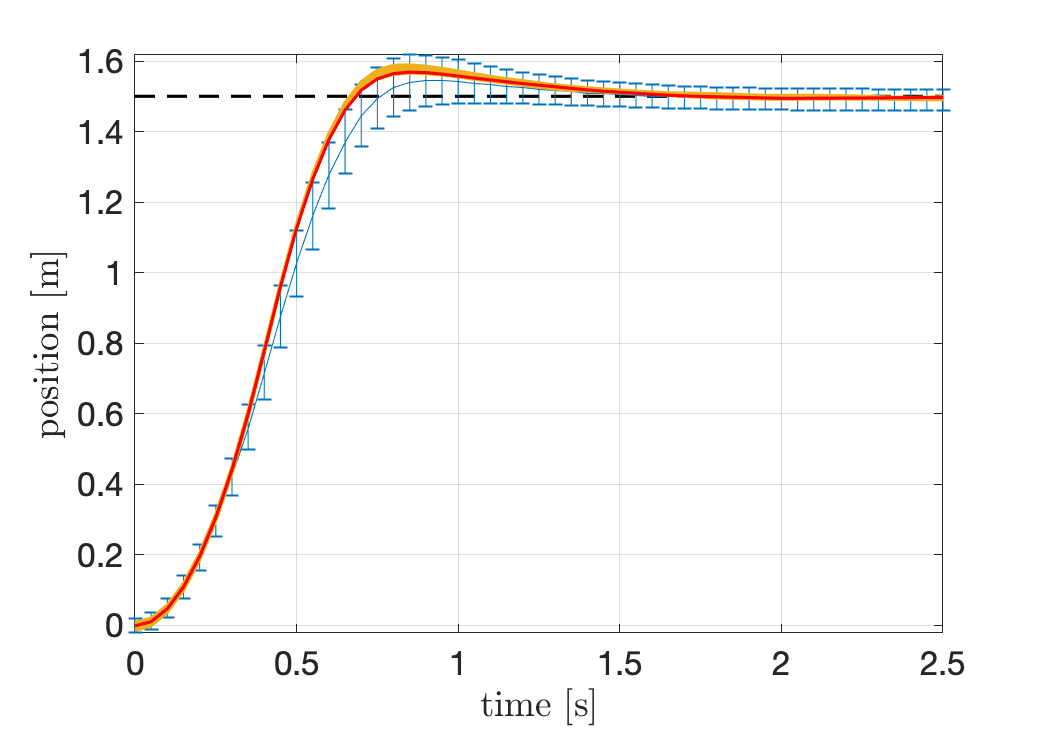
\includegraphics[width=\textwidth]{sdm_quad.png}
	\caption{Spring Damper Mass (trail \#1)\newline}\label{fig:PILCO_sdm}
	\end{subfigure}
	\begin{subfigure}{0.325\textwidth}
	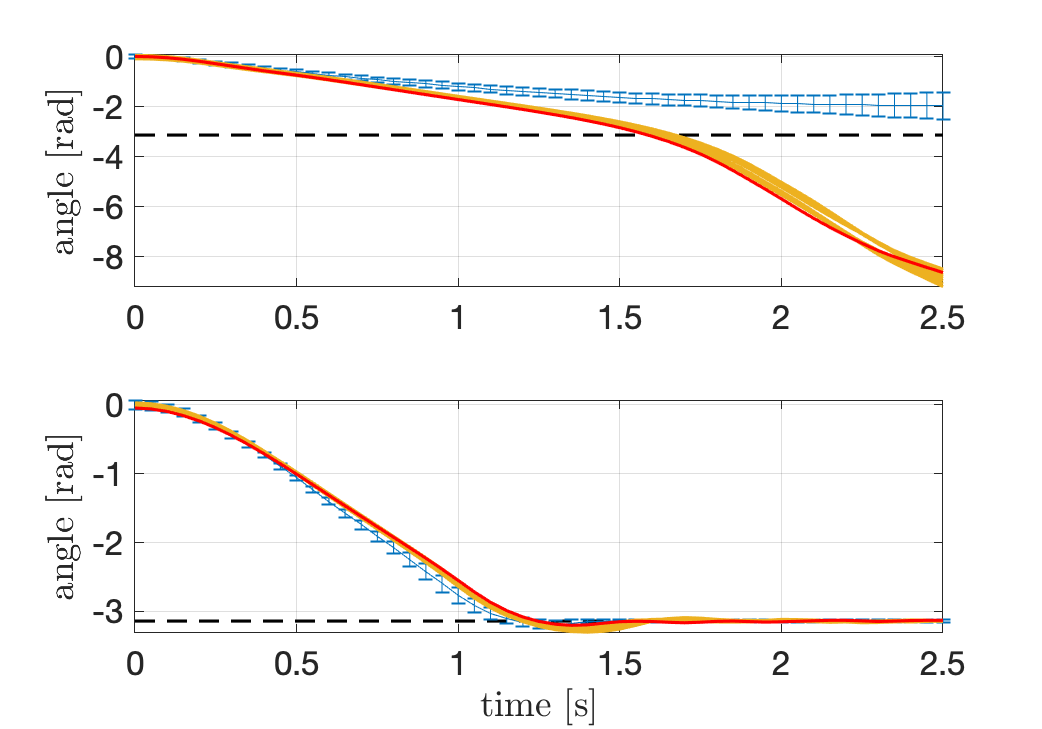
\includegraphics[width=\textwidth]{pend_quad.png}
	\caption{Pendulum (trail \#1 - top, trail \#2 - bottom)\newline}\label{fig:PILCO_pendulum}
	\end{subfigure}
	\begin{subfigure}{0.325\textwidth}
	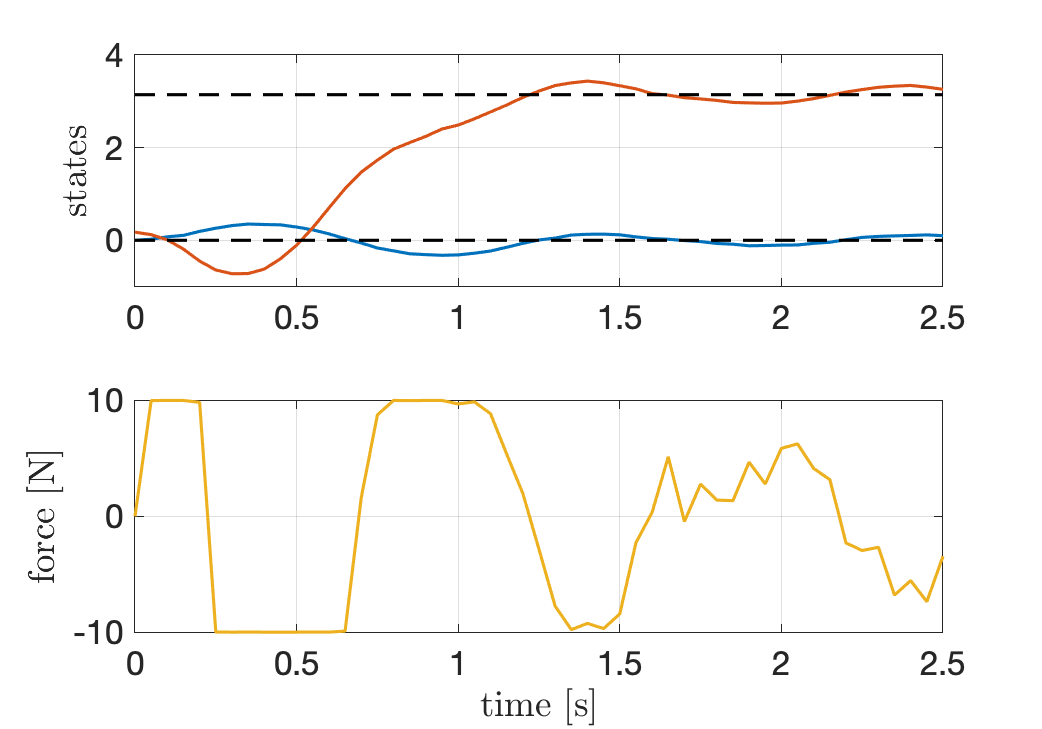
\includegraphics[width=\textwidth]{cp_quad.png}
	\caption{Cart pole, initial angle: 10\textdegree, angle (orange), position (blue), policy (yellow)}\label{fig:PILCO_cp}
	\end{subfigure}\caption{Figures (a)-(b) show trajectories used for training of GP (red), additional rollouts not used for GP training (yellow), predicted system trajectory with confidence interval of 95\% (blue) and target states (black).}\label{fig:PILCO}
\end{figure*} 
\paragraph{Learning Model Dynamics}
The learning of the model dynamics described in equation (\ref{PILCO_sysEq}) is done using a gaussian process (GP), where $\left(x_{t-1},u_{t-1}\right) \in \mathbb{R}^{D+F}$ serve as inputs and $\Delta_t = x_{t} - x_{t-1} + \epsilon \in \mathbb{R}^D$ with $\epsilon \sim \mathcal{N}\left(0,\Sigma_\epsilon\right)$ serve as the GP's outputs. For the GP the squared exponential kernel and a prior mean $m\equiv 0$ is chosen. The parameters (length scales, signal/ noise variance) are trained using evidence maximization. Finally the one step predictions based on the GP are:
\begin{align}
p(x_t\mid x_{t-1}, u_{t-1}) = \mathcal{N} \left(x_t \mid \mu_t, \mathbf{\Sigma}_t \right),\label{PILCO_GPp}\\
\mu_t = x_{t-1} + \mathbb{E}_f \left[ \Delta_t \right],\, \mathbf{\Sigma}_t = \text{var}_f \left[ \Delta_t \right]\label{PILCO_GPmu_sigma}
\end{align}
Here the mean $\mathbb{E}_f\left[\Delta'\right]$ and the variance $\text{var}_f\left[\Delta'\right]$ of a test input $\Delta'$ can be calculated using the GP's hyperparameters\cite{PILCO_paper}.

\paragraph{Policy Evaluation}
In order to predict a successor state $x_t$ based on the policy input $u_{t-1} = \pi\left(x_{t-1},\theta\right)$ a joint distribution $p\left(\tilde{x}_{t-1}\right) = p\left(x_{t-1},u_{t-1}\right)$ has to be determined. This is done by first integrating out the state $x_{t-1}$ where $\mu_u$ and $\mathbf{\Sigma}_u$ are obtained. Secondly by additionally calculating the cross-covariance $\text{cov}_f = \left[{x}_{t-1},u_{t-1}\right]$ the joint state-policy distribution can be approximated by a Gaussian. This result is then used for predicting $p\left(\Delta_t\right)$ with
\begin{equation}\label{PILCO_eq_pDelta}
p\left(\Delta_t\right) = \int p\left(f(\tilde{x}_{t-1})\mid\tilde{x}_{t-1}\right)\, p\left(\tilde{x}_{t-1}\right) \text{d}\tilde{x}_{t-1}
\end{equation}
Often there is no analytically feasible solution for equation (\ref{PILCO_eq_pDelta}). Therefore the Gaussian of $p\left(\Delta_t\right)$ is approximated using moment matching or linearization \cite{GP_deisenroth}. Wtih the Gaussian of $p\left(\Delta_t\right)$ an approximate Gaussian is obtained for $p\left(x_t\right)$ by
\begin{align}
&\mu_t = \mu_{t-1}+\mu_\Delta, \\
&\mathbf{\Sigma}_t = \mathbf{\Sigma}_{t-1} +\text{cov}\left[x_{t-1},\Delta_{t}\right]+\text{cov}\left[\Delta_t,x_{t-1}\right],\\
&\text{cov}\left[x_{t-1},\Delta_{t}\right] = \text{cov}\left[x_{t-1},u_{t-1}\right]\mathbf{\Sigma}_u^{-1}\text{cov}\left[u_{t-1},\Delta_{t}\right].
\end{align}
Finally the the expected cost is calculated according to 
\begin{align}
\mathbb{E}\left[c\left(x_t\right)\right] = \int c\left(x_t\right) \mathcal{N}\left(x_t\mid\mu_t,\mathbf{\Sigma}_t\right) \text{d}x_t.
\end{align}
%where a squared exponential function is preferable, since the gradient is analytically computeable. 
The cost $c(x)$ considering the target state $x_{target}$ is a inverted squared exponential function for each state,
%\begin{equation}
%c\left(x\right) = 1-e^{-\frac{\Vert x-x_{target}\Vert^2}{\sigma_c^2}}
%\end{equation}
where the width is determined by $\sigma_c$.
% determines the width of $c\left(x\right)$.
Using this cost function the resulting partial derivatives over $\mu_t$ and $\Sigma_t$ for the gradients in the policy optimization are calculable in a closed form \cite{GP_deisenroth}.
%Using this cost function the partial derivatives over $\mu_t$ and $\Sigma_t$ for the policy optimization using the gradient 
%\begin{equation}
%\frac{\text{d}\mathbb{E}[c(x_t)]}{\text{d}\theta} = \frac{\partial\mathbb{E}[c(x_t)]}{\partial\mu_t}\frac{\text{d}\mu_t}{\text{d}\theta}+\frac{\partial\mathbb{E}[c(x_t)]}{\partial\Sigma_t}\frac{\text{d}\Sigma_t}{\text{d}\theta}
%\end{equation}
%are calculable in a closed form in (see. \cite{GP_deisenroth}).

%The .
%+Algorithm+
%Implementation is based on the PILCO toolbox which blablabla bla bla

\subsection{Results}
In this part the PILCO algorithm is applied to the three previous introduced systems. The simulations have been done using the online available PILCO framework for MATLAB \cite{PILCO_web}. For the policy a radial basis function (RBF) controller is used. 



Figure \ref{fig:PILCO_sdm} shows that the spring damper mass system is controlled on trail \#1 after optimizing the GP with the data of random exploration in the beginning. This is due to the fact the system is a linear one and the complexity is quite low. 
%The pseudo-control energy used to bring the system to its steady state is 27.1 and the cost of the trajectory is 3.55.
The pendulum in figure \ref{fig:PILCO_pendulum} is controlled after the trial \#2. At trail \#1 the state space of the system is only explored in the angular region from $-\frac{\pi}{2}$ to $\frac{\pi}{2}$. The result is that the GP is only trained with data out of this region and the uncertainty of the GP model grows when the planned trajectory leaves this region (s. blue errorbars in fig. \ref{fig:PILCO_pendulum}). Afer trail \#2 however, the system is stabilized at $-\pi$ for all following trials.
% The trajectories for different inital positions (varying from -0.06 rad to 0.06 rad) are stable as well. 
This shows that PILCO can handle unkown nonlinear systems quite effectively. This becomes even more obvious when considering results of the cart-pole trajectories. It takes 7 trials for the swing up from 10\textdegree, 3 trails from 90\textdegree and 2 trails from 180\textdegree . After the swing up the steady state is controlled stable with slight inaccuarcies. Figure \ref{fig:PILCO_cp} shows the swing up from 10 \textdegree. Remarkable for this  swing up is that  the controller uses gravity to let the pole first swing in the other direction and swing it to its target position afterwards. This is due to  the restriction of the controller to 10 N maximum force. An linear controller would not be able to plan such a trajectory.  %The control energy used for this is XXXX and the cost of the trajectory is YYYY. % It has to be mentioned that accuracy of the steady state highly depends on the GP model's uncertainty, since slight deviations in the policy applied on the model lead to differing system behaviour.


%Pendulum:
%The pendulum is controlled in its target position after only XY trials. Remarkable is the swing up of the pendulum. Afer the first trails the target state is reached, but the controller is instable at that point, since this region of the state space is not predicted correctly by the GP model. But after this region is trained to the GP the controller is able to swing up the pendulum in one step. 
%
%stability in target position
%swing up 
%number of trials
%control energy
%
%
%Cart-pole:
%
%Since the maximum torque is restriced to 10 Nm the pendulum is first swang to the right and then to the left in order to reach its target position. The control energy need for this swing up is XY $\text{Nm}^2$.
%higher dimensional state space needs to be explored
%number of trials/interactions with model
%control energy used
%policy swing up 
%
%Conclusion:
%Computationally expensive , Matrix inversion
%non convex optimization does not guarantee optimal trajectory
%beneficial for unknown systems / no previous knowledge needed

% being applied Spring Damper Mass
%The spring damper mass system is controlled on first trail after sampling data with random exploration noise. Accuarcy is depending on the random exploration noise and sample time (tradeoff). control energy used is determined according to usquare one can see how the model is optimized with the iteration steps
%
%Simulations have been done using the PILCO toolbox 
%In this work a radial basis function (RBF) controller is used.
%+Results+

\section{MODEL-FREE RL}
+Maybe a few sentences about the general idea/concept of model-free RL+
\subsection{Algorithm}

+Algorithm+

\subsection{Results}

+Results+

\section{OPTIMAL CONTROL}
The overarching concept in optimal control is to optimize control inputs and system states according to a specific cost function. 

For linear systems, the method of choice is a linear-quadratic regulator (LQR) that optimizes a linear-quadratic (LQ) cost function. When dealing with non-linear systems, LQR can be iteratively applied to locally LQ problems. This method is called iterative LQR (iLQR). Another method to handle non-linear systems is model-predictive control (MPC). In MPC, an optimization problem to obtain optimal inputs and state trajectories is only solved for a finite time horizon and continually updated during runtime.

For this section, LQR was applied to the linear spring-mass system, iLQR to the pendulum, and MPC to the cart-pole system to highlight the different capabilities of these approaches.
\subsection{Algorithms}


The continuous LQR aims at minimizing the cost function depicted in (\ref{eqn:JanSMcostfunc}).
\begin{equation}\label{eqn:JanSMcostfunc}
	J_1 = \int^{\infty}_{0} \left(x^{T}Q\,x + u^{T}R\,u\right)dt,
\end{equation}
with weight matrices $Q$ and $R$.
Since there was no specifications for input and states, the weights were simply set to $Q=$ diag$(1,1)$ and $R=0.1$. 
This results in an optimal input $u=-K\,x$ which transforms (1) into
\begin{equation}\label{eqn:JanSMcontrolledSys}
	\dot{x} = (A-B\,K)x.
\end{equation}
For the spring-mass system, $K$ was computed using the Matlab function ``lqr''.

Since the goal position is not the origin but rather $x=(1.5 ~ 0)^T$, a prefilter matrix $L$ as shown in (\ref{eqn:JanSMprefilter}) is necessary.
\begin{equation}\label{eqn:JanSMprefilter}
L = \left(C(B\,K-A)^{-1}B\right)^{-1}
\end{equation}
Since LQR is lacking an integral component, a simple PI controller ($K_P=K_I=1$) was added to drive the system into the desired goal position even under disturbances. Note that the system would also be stable for any other controller gain but experience higher overshooting.\\

The iLQR approach for the pendulum was based on [+add reference for Tassa, Mansard and Todorov, 'Control-Limited Differential Dynamic Programming', ICRA 2014+] and their ``iLQG/DDP trajectory optimization'' toolbox for Matlab. 

 To make the problem more interesting, the input is limited to $|u|<4$\,Nm, so that the goal cannot be achieved in a single swing but only by moving back and forth. 

The iLQR (or the similar iLQG) algorithm is a shooting method. This means that an input trajectory is applied to the system (forward pass), and then the input trajectory is optimized (backwards pass). This process is repeated iteratively, until the input trajectory converges.

The cost function for the pendulum problem is defined as 
\begin{equation}\label{eqn:JanPcostfunc}
J_2 = \frac{1}{2}\overline{x}_N^{T}P\,\overline{x}_N + \frac{1}{2}\sum_{k=0}^{N-1}\left(\overline{x}_k^{T}Q\,\overline{x}_k + u_k^{T}R\,u_k\right),
\end{equation}
with the time horizon $N$, the deviation of the current state from the desired state $\overline{x}_k=(x_k-x_{des})$, the final weight matrix $P$, and the familiar $Q$ and $R$ matrices. 

Without any other specifications, the input weight was set to a rather low value of $R=10^{-3}$. 

Even though the desired state is the upright position of the pendulum at zero speed, during the run, only a modest punishment is placed on the correctness of the position to leave enough room for swinging back and forth, and the speed is not punished at all since it is required to drive the pendulum in the desired position. Therefore, this matrix was set to $Q=$ diag$(10^{-3},0)$.

For the final state, the position is the most important factor, while the speed should at least be close to zero, which leads to $P=$ diag$(100,0.1)$.

The iLQR algorithm was set to a time horizon of $N=5000$ at a $t=1$\,ms sample time, which equals a runtime of 5 seconds.

iLQR is an open-loop controller. Therefore, in the implementation, the resulting input trajectory $\underline{u}$ from the optimization was used as feed forward control, while a PID controller minimized the difference between the estimated trajectory $\underline{x}$ (from the optimization) and the actual state.
Without this setup, even the slightest perturbation of the system (e.g. rounding errors) leads to a failed upswing since the goal position is an unstable equilibrium point.\\

 

The MPC implementation was based on the ``nmpc'' function from [+cite Nonlinear Model Predictive Control Theory and Algorithms, Grüne, Lars, Pannek, Jürgen +]. This function aggregates system dynamics, constraints, cost function, and optimization parameters to solve the optimization problem with the Matlab function ``fmincon''.

The input was constrained to $|u|<5$\,N, and the cart position was limited to $|x_1|<4$\,m. The cost function is the same as in (\ref{eqn:JanPcostfunc}), with $P=$ diag$(0,10,10,10)$ (end position of the cart is irrelevant as long as it stays within the bounds), $Q=$ diag$(20,10,10,0)$ (cart should remain in the center during upswing, while angular speed is irrelevant), and $R=0.01$. 

The prediction horizon was set to $N=20$ at a sample time of $t=20$\,ms, and the simulation ran for 4 seconds.

Since MPC is a closed-loop control strategy, no additional controller was necessary.
\subsection{Results}

For the spring-mass system without disturbances, the goal was reach by the LQR controller with $K=$. However, with an added constant disturbance of $d=0.5$\,N, the LQR controller alone fails to reach the desired position, while the addition of the PI controller solves this issue as shown in figure (\ref{fig:JanSM}).
\begin{figure}[htp] 
	\centering
	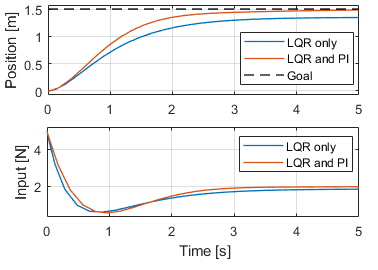
\includegraphics[width=0.5\textwidth]{MS.png}
	\caption{Comparison of LQR and LQR+PI controller. Position $x_1$ of the spring-mass system (top) and control input $u$ (bottom).}
	\label{fig:JanSM}
\end{figure} 

Note that only using the PI controller is not sufficient and would cause the system to become unstable.\\

For the pendulum, the iLQR algorithm converged to a cost of 156.70 after 52 iterations. The resulting trajectory is one initial swing to the left, followed by a complete upswing to the right. This trajectory seems reasonable, since reaching the goal with just a single swing is impossible due to the restrictions on the control input. Figure (\ref{fig:JanP1}) displays the trajectory that the algorithm found and the simulated trajectory with an added PID controller.
\begin{figure}[htp] 
	\centering
	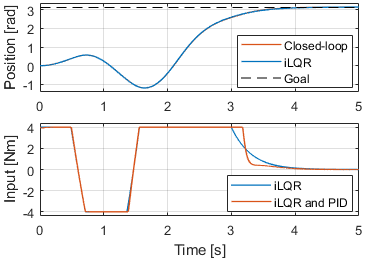
\includegraphics[width=0.5\textwidth]{P1.png}
	\caption{Comparison of iLQR result and closed-loop simulation. Angular position $x_1$ of the pendulum (top) and control input $u$ (bottom).}
	\label{fig:JanP1}
\end{figure} 

Both trajectories are almost identical, and there is only a small deviation in the control input at the end of the upswing (compare figure (\ref{fig:JanP1}) bottom at 3 seconds). However, this slight change is crucial to keep the pendulum in the upright position. Without the added PID controller, the system remains instable as shown in figure (\ref{fig:JanP2}), since iLQR is not a closed-loop controller.
\begin{figure}[htp] 
	\centering
	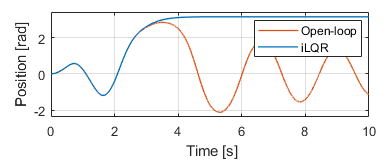
\includegraphics[width=0.5\textwidth]{P2.png}
	\caption{Comparison of iLQR result and open-loop simulation. Angular position $x_1$ of the pendulum.}
	\label{fig:JanP2}
\end{figure}\\

The MPC controller managed to stabilize the pendulum of the cart-pole in the upright position after 135 time steps or 2.7 seconds. Due to the input constraints, the car had to move left and right a few times to allow the pendulum to swing back and forth until it reached the upright position. The successful swing-up is presented in figure (\ref{fig:JanCP}). 
 \begin{figure}[htp] 
 	\centering
 	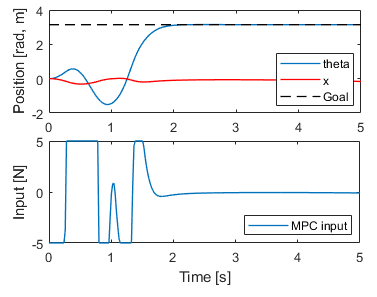
\includegraphics[width=0.5\textwidth]{CP.png}
 	\caption{The swing-up of the cart-pole system. Angular position $\theta=x_3$ of the pendulum and horizontal displacement $x=x_1$ of the car (top) and control input $u$ (bottom).}
 	\label{fig:JanCP}
 \end{figure}

Since MPC is a closed-loop control strategy, the system remained in the upright position after reaching it initially.

\section{COMPARISON AND DISCUSSION}
+TBD+

\section{CONCLUSION}
+TBD+



\begin{thebibliography}{99}

\bibitem{PILCO_paper} Deisenroth, Marc, and Carl E. Rasmussen. "PILCO: A model-based and data-efficient approach to policy search." Proceedings of the 28th International Conference on machine learning (ICML-11). 2011.
\bibitem{GP_deisenroth} Deisenroth, Marc Peter, Dieter Fox, and Carl Edward Rasmussen. "Gaussian processes for data-efficient learning in robotics and control." IEEE transactions on pattern analysis and machine intelligence 37.2 (2015): 408-423.
\bibitem{PILCO_web} Deisenroth, Marc Peter, Dieter Fox, and Carl Edward Rasmussen. "PILCO website", 2013. [Online]. Available: http://mlg.eng.cam.ac.uk/pilco/. [Accessed: 27- Jan- 2019]

%\bibitem{c1} G. O. Young, ÒSynthetic structure of industrial plastics (Book style with paper title and editor),Ó 	in Plastics, 2nd ed. vol. 3, J. Peters, Ed.  New York: McGraw-Hill, 1964, pp. 15Ð64.
%\bibitem{c2} W.-K. Chen, Linear Networks and Systems (Book style).	Belmont, CA: Wadsworth, 1993, pp. 123Ð135.
%\bibitem{c3} H. Poor, An Introduction to Signal Detection and Estimation.   New York: Springer-Verlag, 1985, ch. 4.
%\bibitem{c4} B. Smith, ÒAn approach to graphs of linear forms (Unpublished work style),Ó unpublished.
%\bibitem{c5} E. H. Miller, ÒA note on reflector arrays (Periodical styleÑAccepted for publication),Ó IEEE Trans. Antennas Propagat., to be publised.
%\bibitem{c6} J. Wang, ÒFundamentals of erbium-doped fiber amplifiers arrays (Periodical styleÑSubmitted for publication),Ó IEEE J. Quantum Electron., submitted for publication.
%\bibitem{c7} C. J. Kaufman, Rocky Mountain Research Lab., Boulder, CO, private communication, May 1995.
%\bibitem{c8} Y. Yorozu, M. Hirano, K. Oka, and Y. Tagawa, ÒElectron spectroscopy studies on magneto-optical media and plastic substrate interfaces(Translation Journals style),Ó IEEE Transl. J. Magn.Jpn., vol. 2, Aug. 1987, pp. 740Ð741 [Dig. 9th Annu. Conf. Magnetics Japan, 1982, p. 301].
%\bibitem{c9} M. Young, The Techincal Writers Handbook.  Mill Valley, CA: University Science, 1989.
%\bibitem{c10} J. U. Duncombe, ÒInfrared navigationÑPart I: An assessment of feasibility (Periodical style),Ó IEEE Trans. Electron Devices, vol. ED-11, pp. 34Ð39, Jan. 1959.
%\bibitem{c11} S. Chen, B. Mulgrew, and P. M. Grant, ÒA clustering technique for digital communications channel equalization using radial basis function networks,Ó IEEE Trans. Neural Networks, vol. 4, pp. 570Ð578, July 1993.
%\bibitem{c12} R. W. Lucky, ÒAutomatic equalization for digital communication,Ó Bell Syst. Tech. J., vol. 44, no. 4, pp. 547Ð588, Apr. 1965.
%\bibitem{c13} S. P. Bingulac, ÒOn the compatibility of adaptive controllers (Published Conference Proceedings style),Ó in Proc. 4th Annu. Allerton Conf. Circuits and Systems Theory, New York, 1994, pp. 8Ð16.
%\bibitem{c14} G. R. Faulhaber, ÒDesign of service systems with priority reservation,Ó in Conf. Rec. 1995 IEEE Int. Conf. Communications, pp. 3Ð8.
%\bibitem{c15} W. D. Doyle, ÒMagnetization reversal in films with biaxial anisotropy,Ó in 1987 Proc. INTERMAG Conf., pp. 2.2-1Ð2.2-6.
%\bibitem{c16} G. W. Juette and L. E. Zeffanella, ÒRadio noise currents n short sections on bundle conductors (Presented Conference Paper style),Ó presented at the IEEE Summer power Meeting, Dallas, TX, June 22Ð27, 1990, Paper 90 SM 690-0 PWRS.
%\bibitem{c17} J. G. Kreifeldt, ÒAn analysis of surface-detected EMG as an amplitude-modulated noise,Ó presented at the 1989 Int. Conf. Medicine and Biological Engineering, Chicago, IL.
%\bibitem{c18} J. Williams, ÒNarrow-band analyzer (Thesis or Dissertation style),Ó Ph.D. dissertation, Dept. Elect. Eng., Harvard Univ., Cambridge, MA, 1993. 
%\bibitem{c19} N. Kawasaki, ÒParametric study of thermal and chemical nonequilibrium nozzle flow,Ó M.S. thesis, Dept. Electron. Eng., Osaka Univ., Osaka, Japan, 1993.
%\bibitem{c20} J. P. Wilkinson, ÒNonlinear resonant circuit devices (Patent style),Ó U.S. Patent 3 624 12, July 16, 1990. 






\end{thebibliography}




\end{document}